% --------------------------------------------------------------------------- %
%            _       _                 _            _   _                     %
%           (_)_ __ | |_ _ __ ___   __| |_   _  ___| |_(_) ___  _ __          %
%           | | '_ \| __| '__/ _ \ / _` | | | |/ __| __| |/ _ \| '_ \         %
%           | | | | | |_| | | (_) | (_| | |_| | (__| |_| | (_) | | | |        %
%           |_|_| |_|\__|_|  \___/ \__,_|\__,_|\___|\__|_|\___/|_| |_|        %
% --------------------------------------------------------------------------- %
\chapter{Augmented Reality as Medium for Sound ARt Composition and Performance}
\label{sec: introduction}
\epigraph{\emph{Music, which should pulsate with life, needs new means of expression, and science alone can infuse it with youthful vigor.}}{\citep{varese1966}}

\begin{figure}
    \centering
    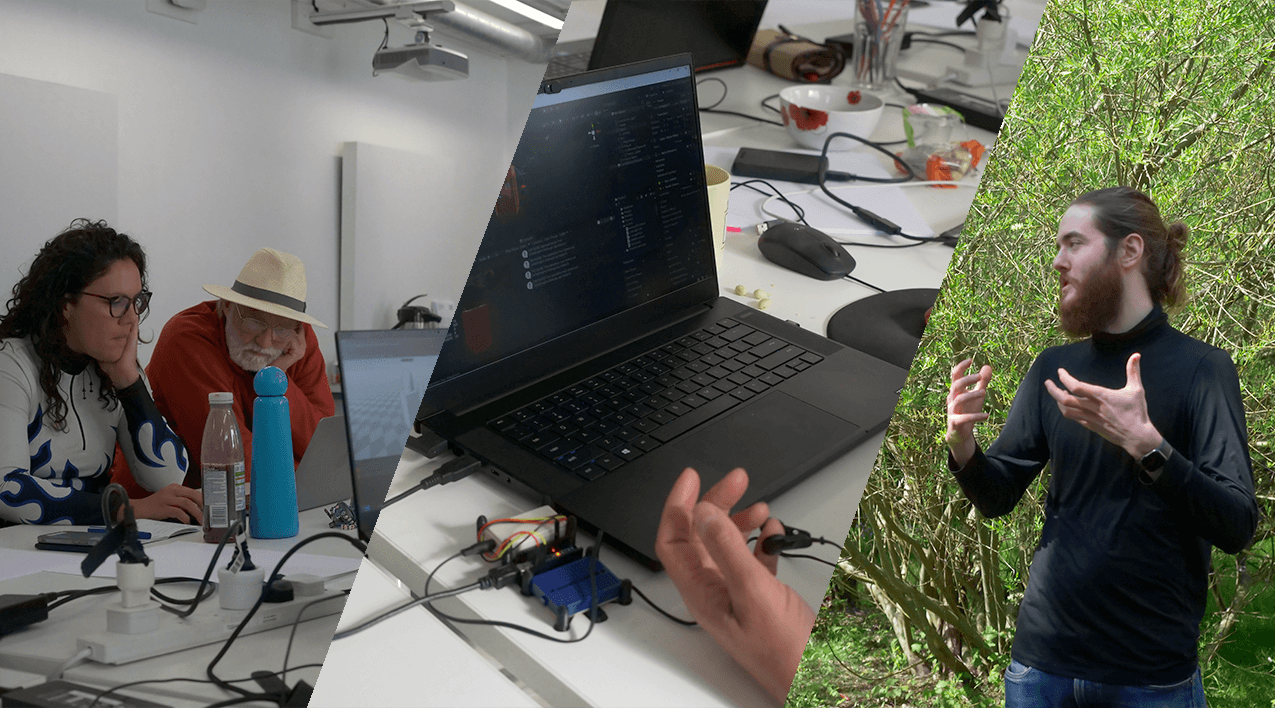
\includegraphics[width=1\linewidth]{01-intro/chapter-fig.png}
    \captionsetup{labelformat=empty}
    \caption[\autoref*{sec: introduction}'s page-figure: \textit{polygons\textasciitilde{}} in performance at the Attenborough Centre for Creative Arts, University of Sussex, on June 8th, (from \citeauthor{bilbow2022a}, \citeyear{bilbow2022a})]{}
\end{figure}

\clearpage
% --------------------------------------------------------------------------- %
\section{Summary}\label{sec: introduction-summary}

In the last twenty years, computational technology has become more and more expressive, the systems we engage with becoming increasingly interactive. Due to this, the arts, including forms of digital sound art, have embraced new technologies in tandem with, and often contributing to, their development. This has led to more human-centred methods of designing tools of digital art creation, moving away from black-boxed (undisclosed to the audience) interactions, towards more performative and suggestive interactions, which often include the audience. Among some of the technologies that have seen nascent use in the arts is \gls{xr} \footnote{The meaning of `X' in \gls{xr} is a hotly contested topic, check its term entry for more on its definition}, a group of technologies that promise to radically rethink the way we approach digital and physical reality. 

The category of \gls{xr} is comprised of: \gls{vr} - technology that promises to immerse us in a completely synthetic virtual world; and \gls{ar} - technology that promises to immerse us in our own real world through the computational mediation of virtual processes \footnote{The present thesis makes no distinction between \gls{mr} and \gls{ar}, and adopts \gls{ar} as an umbrella term for all contemporary (and mostly marketing) uses of the term \gls{mr}. Check the glossary for more on the distinctions others make between the two terms}. This leads to the augmentation, diminution, hybridisation, or extension of our own experience of reality, blurring and perhaps dissolving the line between our virtual and real selves.

\gls{ar}, as mentioned, has seen sporadic use in the arts in the last twenty years. Its use in other disciplines, such as medical science, manufacturing and repair, annotation and visualisation, and the military \citep{azuma1997}, have been typically characterised by its use as technology that aids or facilitates the \textbf{visual overlay and alignment} of \textbf{virtual graphics} (text, image, animation, video) onto our \textbf{real world environment}. Within these fields, this has a potential myriad important uses, from training junior doctors in dummy procedures by overlaying the steps of a difficult surgery, to allowing three-dimensional networked collaboration across vast distances. Within the arts, its use has also been typically limited to this `visual overlay' approach. Despite being only a fraction of the possible forms of \gls{ar}, this conception of \gls{ar} dominates the market of consumer \gls{ar} devices, from head-mounted, to handheld and projective technologies, the majority deal with overlaying visual information. 

By taking a \gls{diy} approach to designing and implementing custom digital musical tools through hardware and software in \autoref{sec: method}, the present practice-based research thesis approaches \gls{ar} through a multisensory lens to designing rich, expressive experience. The importance of such an approach is in its ability help redefine, and understand more about the technologies with which we are choosing to mediate our daily lives with, considering their origins, and also about how our own perception of digital media is affected through this embodied usage. 



% --------------------------------------------------------------------------- %
\section{Personal Motivations}\label{sec: introduction-motivations}
My own motivations for taking this approach \gls{ar} experience is in the potential for it to afford creative, rich, sensory artwork, which seeks to teach us more about the way we perceive ourselves, others, and our environment. Coming from a background in music technology, specifically in developing and evaluating digital music tools and instruments, the nature of typical `visual overlay' \gls{ar} is seemingly incompatible with its use as a digital music tool. As such, it seems not only possible, but reasonable for it to be redefined to encapsulate all senses, and processes of perceptual modulation. In wanting to foster embodied experience between audience members (collaborative expression), \gls{ar} offers a unique way of mediating and co-constructing the space in which they embody. Thus, my motivation is also within the advancement of our understanding this hybrid space, in which unique relationships between virtual and real processes are played out.



% --------------------------------------------------------------------------- %
\section{Key Research Questions}\label{sec: introduction-researchquestions}
\gls{ar} has seen nascent implementation as a creative medium in the arts, and more specifically music composition and performance. Therefore, the research areas and questions for the present thesis are based in the intersection between the arts, technology, sensory perception:

\RQall

% --------------------------------------------------------------------------- %
\section{Aims \& Objectives of the Thesis}\label{sec: introduction-aims}
As well as answering and contributing understanding to the above research questions, this thesis aims to:

\begin{itemize}
    \item Conduct a thorough literature and practice review of the field of \gls{ar} generally and within the arts
    \item Apply theories of materiality, embodiment, and space to contemporary \gls{ar} design, use, and evaluation.
    \item Contribute to the practice field of \gls{ar} sound arts by designing and evaluating \gls{ar} experiences for creative and collaborative expression.
    \item Contribute to the understanding of how such tools might affect our perceptions of self, others and our real, virtual, and hybrid environments. 
    \item Propose workflows that may help artists and musicians interested in leveraging \gls{ar} within sound art composition and performance
\end{itemize}



% --------------------------------------------------------------------------- %
\section{Research Methods}\label{sec: introduction-methods}
The research methods used to answer my research questions, and achieve my aims and objectives above involve taking a practice-based approach to designing multisensory digital musical instruments using \gls{ar}. Much of this is grounded in a resistance to the origin of \gls{ar} from within the U.S. military-industrial complex, and the effects this has had on the typical form of \gls{ar} found today. In developing three sound \gls{art} experiences, I qualitatively (coded interview) evaluating these instruments and tools, and iteratively redesigning them to provide rich and immersive experience to myself as well as participants. This iteration has led to theoretical implications for the sonic medium found in \autoref{sec: discussion-medium}, and a set of reproducible design patterns for artists and musicians interested in using \gls{ar} creatively in \autoref{sec: discussion-patterns}.




% --------------------------------------------------------------------------- %
\section{Outline of Chapters}\label{sec: introduction-outline}
\autoref{sec: review} starts with an genealogy of \gls{ar} as an emerging technology within the field of \gls{hci}, examining the effects that historical barriers to usage such as portability, price, as well as its origination in the military-industrial complex, have had on typical forms today. Among these forms, it is found that the majority deal with simple and descriptive visual additions in the form of text, image, animation or video overlay. I make a case for `multisensory' \gls{ar}, i.e. the designing of content or experience for multiple senses to counter not only this bias toward visual design, but also as a method of attaining richer and more novel experiences of \gls{ar}. This case is made by examining current advancements in multisensory \gls{hci} applications and enabling technologies. In the second part of the chapter, I posit through a review of contemporary art practice, the potential of \gls{ar} use within the arts in contributing to the designing and evaluation of expressive tools, enabling new aesthetic and multisensory experiences, collaborative expression, and agency.

In \autoref{sec: theory}, I outline the position the thesis takes regarding aesthetic experience and artistic production, as well as outlining a key contemporary theory of mind (the `4 E's') that may help explicate aesthetic experience in \gls{ar}. I identify three lenses through which to view, not only the potential of modern-day applications of sound \gls{art}, but also the potential of the medium itself. The first is through a consideration of the materiality and form of complex processes in \glspl{dmi} and interactive music systems for designers, performer, and audience. The second is through examining of current theories of enactivism in action within \gls{xr} technologies. The last is through considering the intervention of \gls{ar} processes in real and virtual spaces, how this effects the construction of these spaces, the implications this in-turn has for the type of art that is created, and the privacy and security of people co-located in these spaces - is the Metaverse really where we want our \gls{art} to exist and be `consumed'? 

\autoref{sec: method} contains the methodology through which I address my research questions, this is separated into three sections. First, I contextualise the methodological approach taken within the findings of the previous two chapters. Secondly, an outlining of the concept of resistance, which has guided and motivated my practical and theoretical work towards \glsfirst{opensource} technologies, non-visual sensory displays, and the processual nature of \gls{ar}'s ability to modulate perception. Thirdly, I examine individually the methods taken in the ensuing three study chapters.
 
In \autoref{sec: area}, I outline the development and evaluation of the \textit{area\textasciitilde{}} system. \textit{area\textasciitilde{}} enables users to record, manipulate, and spatialise virtual audio samples or nodes around their immediate environment. Through a combination of ambisonics audio rendering and hand gesture tracking, this system calls attention to the ability of non-visual \gls{ar}, here, audio \gls{ar}, to provide new aesthetic experiences of real and virtual environments. Through an \gls{abd} study, this pilot study proposes that rich experience can result from non-visual \gls{ar} systems. 

\autoref{sec: polaris} describes the design, experience, and evaluation of an \gls{av} \gls{ar} piece called {polaris\textasciitilde{}}, developed using mainly \gls{floss} and \gls{osh}. Studies took place in October 2021, and the experiences of 10 participants were analysed using the grounded theory analysis method to draw out commonalities. In evaluating \textit{polaris\textasciitilde{}} it was found that the experience engaged participants fruitfully, with many noting their ability to express themselves audiovisually in creative ways. The remarks from the transcriptions of these studies, that were then sorted into the categories of Sentiment, Learning, Adoption, Expression, and Immersion. 

\autoref{sec: polygons} outlines my journey deploying \gls{ar} as a tool for sound \gls{art} performance, detailing problems, solutions, and the experience of performing the piece \textit{polygons\textasciitilde{}} in \gls{ar}. The performance was the first time I had immersed myself in the \textit{polygons\textasciitilde{}} system for an extended period of time which lead to an authentic exploration and improvisation of the material, embodied, and spatial affordances of the three instruments in the system \textit{ambi}, \textit{click+-}, and \textit{hands}.

\autoref{sec: discussion} briefly reviews the positionality of the thesis as carved out in \autoref{sec: review} and \autoref{sec: theory}, before discussing the \gls{diy} method outlined in \autoref{sec: method}. Combined results of the three studies are highlighted, and implications for the sonic medium of \gls{ar} are proposed. Then, I propose a set of design patterns through which artists and musicians in the field can produce expressive works using \gls{ar}. The thesis is concluded in \autoref{sec: conclusion} with final thoughts, future recommendations, and contributions outlined.
